\section{Uncertainty and Robustness}

In this section the uncertainty model will be derived to include various aspects where uncertainly is present.

Looking at the method in which the model is derived, the main uncertainties in this description of the process are

\begin{enumerate}
	\item  Parametric uncertainty. This is from the fact that the model is fitted. The variables used for fitting the models were rounded to produce numbers that are easy to work with. This causes uncertainty regarding the accuracy of the model, as all the variables may be wrong by a fractional amount.
	\item Uncertainty due to neglected dynamics. This will most certainly be included in the current model, as the core principle behind fitting dynamic models to experimental data involves the simplification of multi order differential equations to first or second order systems. 
\end{enumerate}

The above list contains the uncertainties that are certain. Some uncertainties are unlikely. These uncertainties will not be considered when deriving the uncertainty model. This includes

\begin{enumerate}
	\item Neglected delays. This can be excluded, as all the modelled equations contains delays. The uncertainty regarding the delays will therefore only be analysed when looking at the parametric uncertainty of the values of $\theta_{ij}$.
\end{enumerate}

\subsection{Choosing the Uncertainty Weight Form}

A major thing to consider when setting up the uncertainty model is which uncertainty weight form to use. The two major weights to choose from are

\begin{enumerate}
	\item Additive uncertainty.
	\item Multiplicative weight uncertainty.
\end{enumerate}

The major deciding factor for the choice will be the ease of fitting the uncertainty weight to the smallest uncertainty radius of all possible plants ($\Pi$). In mathematical terms the radius can be described as 
\begin{equation}
	l_A = \max_{G_p \epsilon \Pi} |G_p(j\omega) - G(j\omega)|
\end{equation}

for additive uncertainty, and 

\begin{equation}
	l_I = \max_{G_p \epsilon \Pi} |\frac{G_p(j\omega) - G(j\omega)}{G(j\omega)}|
\end{equation}

for multiplicative uncertainty. In the above equations $G_p(j\omega)$ refers to the perturbed model. The complete uncertainty analysis was pulled from \textcite{skogestad}, and for more information regarding the concepts please consult the reference material. Preferably the uncertainty weight should have the lowest possible order. The relative shape difference between the two uncertainty descriptions are displayed in Figure~\ref{fig:uncertaintyadditivevsmultiplicative}.

\begin{figure}[H]
	\centering
	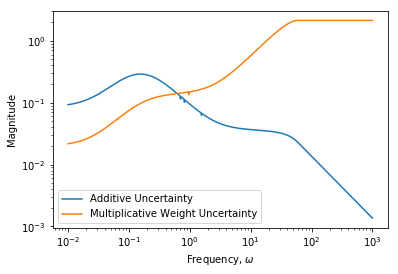
\includegraphics[width=0.7\linewidth]{Figures/Uncertainty_Additive_vs_Multiplicative}
	\caption{A comparison between additive and multiplicative uncertainty weight requirements, when analysing parametric uncertainty of a first order plus dead time equation.}
	\label{fig:uncertaintyadditivevsmultiplicative}
\end{figure}

From the picture it is clear that drastically different shapes for $l_A$ and $l_I$ is obtained using the uncertainty descriptions. When the two are compared, it is clear that

\begin{enumerate}
	\item The additive uncertainty will require at least one lead and two lag term to get an acceptable fit. Only using one lag will lead to an over estimated uncertainty for low frequencies. To gain an even tighter fit one additional lag and lead term can be added. This however will result in a very complex uncertainty weight.
	\item The multiplicative uncertainty requires only one lag and one lead to get an acceptable fit. For a tighter fit, one additional lag and lead can be added. This is not entirely necessary, as the frequencies where uncertainty is over estimated are in the crossover frequency range. This is therefore a very conventional fit. In later sections the benefit of this estimation with regard to unmodelled dynamics uncertainty is discussed. 
\end{enumerate}

For this uncertainty description multiplicative weights will be used to describe the uncertainty. This is simply due to the ease of fitting the multiplicative weights to the uncertainty descriptions.

\subsection{Parametric Uncertainty}

As mentioned in the previous section, parametric uncertainty is inherent to the model. Using the data and subsequent models fit to the data, is was decided to

\begin{itemize}
	\item Estimate the uncertainty of all gains as 2 \%.
	\item Estimate the uncertainty of all time constants as 10 \%.
	\item Estimate the uncertainty of all time delays as 2 \%.
\end{itemize}

The values above are chosen based on the distribution of data points in key places, during the step test analysis. The steady state gains were relatively clear due to a small variance distribution of particles along the horizontal lines (steady state) in the time domain responses. The same principle applies to the time it takes before a response is observed. The critical point is quite easily identifiable, and the first order plus dead time models can capture the dead time in the system with little uncertainty regarding the value of the dead time. This is most definitely due to high quality measuring devices that can deliver consistent accurate measured values.

It is only in the middle of the step responses that a deviation in measured value occurred. This is captured in a lower local $R^2$ value in this region of the step response. This is the reason why the time constants are more uncertain than the other parameters.

All the first order plus dead time transfer functions within $G(s)$ have the relatively the same shape (their uncertainty descriptions are the same). For this reason, the same fitting function was used to describe the performance weights. This function is

\begin{equation}
	\label{eq:Uncertainty weights}
	w_{Ii} = \frac{Ts + k_1}{(T/2.5)s + 1}
\end{equation}

This is the minimum order uncertainty weight that could be fit to the functions, and was chosen to simplify the uncertainty model. Table~\ref{tab:Uncertainty description G(s)} contains all the various constants for the uncertainty model of $G(s)$.

\begin{table}[H]
	\centering
	\begin{tabular}{cccc}
		\hline
		\textbf{Transfer Function} & \textbf{Uncertainty Weight} & \textbf{$T$} & \textbf{$k_1$} \\
		\hline
		$G_{11}$                        & $w_{I11}$                  & 0.7        & 0.02        \\
		$G_{12}$                        & $w_{I12}$                  & 0.5        & 0.015       \\
		$G_{13}$                        & $w_{I13}$                  & 0.55       & 0.04        \\
		$G_{21}$                        & $w_{I21}$                  & 0.3        & 0.06        \\
		$G_{22}$                        & $w_{I22}$                  & 0.2        & 0.05        \\
		$G_{23}$                        & $w_{I23}$                  & 0.75       & 0.035       \\
		$G_{31}$                        & $w_{I31}$                  & 0.07       & 0.09        \\
		$G_{32}$                        & $w_{I32}$                  & 0.05       & 0.1       \\\hline 
	\end{tabular}
	\caption{The uncertainty model of the first order plus dead time components of $G(s)$}
	\label{tab:Uncertainty description G(s)}
\end{table}

Figure~\ref{fig:Uncertainty wI 11} and Figure~\ref{fig:Uncertainty wI 13} graphically illustrates the procedure of fitting the uncertainty curves. The complete set of fitted figures can be found in the Appendix.

\begin{figure}[H]
	\centering
	\begin{minipage}{.48\textwidth}
		\centering
		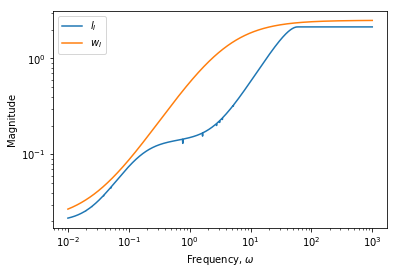
\includegraphics[width=\linewidth]{Figures/Uncertainty_wI_11}
		\captionof{figure}{The uncertainty weight of transfer function $G_{11}$.}
		\label{fig:Uncertainty wI 11}
	\end{minipage}%
	\hfill
	\begin{minipage}{.48\textwidth}
		\centering
		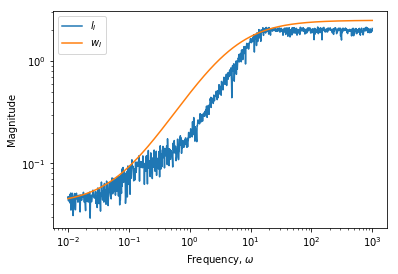
\includegraphics[width=\linewidth]{Figures/Uncertainty_wI_13}
		\captionof{figure}{The uncertainty weight of transfer function $G_{13}$.}
		\label{fig:Uncertainty wI 13}
	\end{minipage}
\end{figure}

From Figure~\ref{fig:Uncertainty wI 13} it is apparent that the optimization function used to solve the "worst case" combination of the parameters did not return a smooth solution. Increasing the number of start for the optimization function had no effect. In fact, al the functions with negative gain did not return a smooth curve when passed to the optimization function. Unfortunately, due to time constraints, the matter could not be investigated any further. The performance weight was just adjusted to lie on the top part of the fluctuating curve.

The transfer function $G_{33}$, required special attention, as this was not simply a first order plus dead time model. There are more time constants (a total number of three) in the function. All variables carried the same uncertainty as specified above. The ultimate performance weight function was determined as

\begin{equation}
	w_{I33} = \frac{(0.8s + 8)(0.55s + 0.0095)}{(11s + 1)(0.015s + 1)}
\end{equation}

The fitting of the uncertainty weight to $l_I$ is displayed in Figure~\ref{fig:uncertaintywi33}.

\begin{figure}[H]
	\centering
	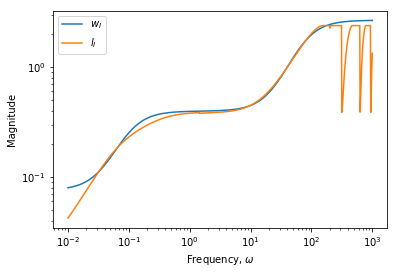
\includegraphics[width=0.7\linewidth]{Figures/Uncertainty_wI_33}
	\caption{The uncertainty weight of transfer function $G_{33}$.}
	\label{fig:uncertaintywi33}
\end{figure}

A much tighter uncertainty weight fit was achieved using this model. The weight described in Equation~\ref{eq:Uncertainty weights} was too inaccurate. Big over estimates would have been made at very low frequencies, as well as at crossover frequencies.

The same procedure was carried out to construct an uncertainty model for $G_d(s)$. There were again a lot of first order plus dead time elements in the system. Equation~\ref{eq:Uncertainty weights} was used to fit all of the multiplicative uncertainty descriptions. Table contains the resulting calculated constants.

\begin{table}[H]
	\centering
	\begin{tabular}{cccc}
		\hline
		\textbf{Transfer Function} & \textbf{Uncertainty Weight} & \textbf{$T$} & \textbf{$k_1$} \\
		\hline
		$G_{d11}$                        & $w_{Id11}$                  & 1.5        & 0.01        \\
		$G_{d21}$                        & $w_{Id21}$                  & 0.8        & 0.015        \\
		$G_{d31}$                        & $w_{Id31}$                  & 0.8       & 0.015        \\
		$G_{d32}$                        & $w_{Id 32}$                 & 0.8       & 0.015       \\\hline 
	\end{tabular}
	\caption{The uncertainty model of the first order plus dead time components of $G_d(s)$}
	\label{tab:Uncertainty description Gd(s)}
\end{table}

In $G_d(s)$ there are also two transfer function equation that are more complicated. The multiplicative uncertainty form has a shape that will require two lags and two leads in an uncertainty weight. The additive uncertainty form however only requires two lags and one lead. The uncertainty form slected for these two elements was therefore the additive form. The uncertainty weights calculated are

\begin{equation}
	w_{A12} = \frac{6.94(-0.3s+1)}{(s+1)^2}
\end{equation}

and 

\begin{equation}
w_{A22} = \frac{11(35s+1)}{(9.65s+1)^2}
\end{equation}

Figure~\ref{fig:Uncertainty wI Gd12} and Figure~\ref{fig:Uncertainty wI Gd22} displays the uncertainty weights fit for the above two equations.

\begin{figure}[H]
	\centering
	\begin{minipage}{.48\textwidth}
		\centering
		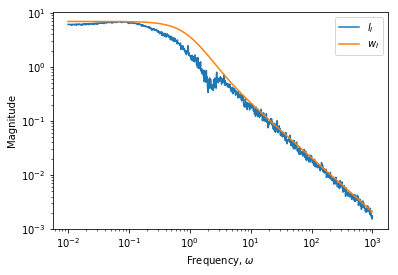
\includegraphics[width=\linewidth]{Figures/Uncertainty_wI_Gd12}
		\captionof{figure}{The uncertainty weight of transfer function $Gd_{12}$.}
		\label{fig:Uncertainty wI Gd12}
	\end{minipage}%
	\hfill
	\begin{minipage}{.48\textwidth}
		\centering
		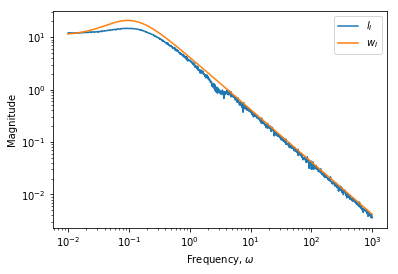
\includegraphics[width=\linewidth]{Figures/Uncertainty_wI_Gd22}
		\captionof{figure}{The uncertainty weight of transfer function $Gd_{22}$.}
		\label{fig:Uncertainty wI Gd22}
	\end{minipage}
\end{figure}